\documentclass[11pt,a4paper]{article}
\usepackage[margin=1in]{geometry}
\usepackage{amsmath,amssymb,amsthm,bm}
\usepackage{lmodern}\usepackage[T1]{fontenc}\usepackage{graphicx,booktabs,hyperref,xcolor}\usepackage[expansion=false]{microtype}
\usepackage[font=small,labelfont=bf]{caption}
\usepackage{array}
\usepackage{placeins}
\renewcommand{\topfraction}{0.9}\renewcommand{\bottomfraction}{0.7}\renewcommand{\textfraction}{0.08}\renewcommand{\floatpagefraction}{0.75}
\setcounter{topnumber}{3}\setcounter{bottomnumber}{2}\setcounter{totalnumber}{4}
\newcommand{\SI}[2]{\ensuremath{#1\,\mathrm{#2}}}\newcommand{\SIrange}[3]{\ensuremath{#1\text{--}#2\,\mathrm{#3}}}
\usepackage[numbers,sort&compress]{natbib}
\hypersetup{colorlinks=true,linkcolor=blue!60!black,citecolor=blue!60!black,urlcolor=blue!60!black}
\graphicspath{{../results/figs/}}
\newtheorem{theorem}{Theorem}\newtheorem{lemma}[theorem]{Lemma}\newtheorem{proposition}[theorem]{Proposition}
\newtheorem{corollary}[theorem]{Corollary}\theoremstyle{remark}\newtheorem*{remark}{Remark}
\newcommand{\R}{\mathbb{R}}\newcommand{\C}{\mathbb{C}}\newcommand{\PSD}{\succeq 0}
\DeclareMathOperator{\Tr}{Tr}\DeclareMathOperator{\rank}{rank}\DeclareMathOperator{\conj}{conj}
\newcommand{\I}{I}\newcommand{\rhostar}{\rho^{\star}}
\newcommand{\NA}{\mathrm{NA}}
\newcommand{\EL}{\mathrm{EL}}

\title{Certified Bounds for Partially Coherent Mask Synthesis:\\ Convex Printability Certificates, Rigorously Separated Single- and Multi-Exposure Optima, and Pattern-Specific Exposure-Latitude Limits}
\author{Author names withheld (autonomous research system with human oversight)\thanks{Code, data and the full verification record are available in the accompanying repository (\texttt{code/}, \texttt{results/}, \texttt{notes/}). Every number in this manuscript is produced by \texttt{code/run\_all\_par.sh} from scratch.}}
\date{October 12, 2026 --- manuscript v2 (internally verified; not peer reviewed)}

\sloppy
\begin{document}\maketitle

\begin{abstract}
\noindent\textbf{Purpose.} Mask synthesis for projection lithography (ILT, SMO) is nonconvex, so a local optimum says nothing about the best achievable image. We provide solver-independent limits on printability.

\noindent\textbf{Methods.} For the Abbe/Hopkins model of a periodic cell---scalar or vector, with arbitrary aberrations and focus sets---the best achievable dark-to-bright intensity ratio $\rhostar$ (equivalently, the maximum exposure latitude) is bounded by a semidefinite relaxation in the diffraction-order domain. Its dual is a certificate: nonnegative weights on dark and bright sample points such that one matrix is positive semidefinite, verified independently of the solver and rigorized against round-off. We prove that the relaxation equals the unlimited-multiple-exposure problem, that nonnegative one-dimensional masks form the Carath\'eodory--Toeplitz cone, and that pixelation at or above the collected-order count leaves the bound unchanged. An interval branch-and-bound certifier bounds the single-mask optimum.

\noindent\textbf{Results.} The bound reproduces the $k_1$ cutoffs for DUV and EUV. On 109 random one-dimensional targets, local optimization is certified globally optimal in 70\% of cases and within 1\% in 83\%; all two-dimensional contact arrays are certified within 0.3\%, and two of three \SI{320}{nm} T-junction and line-end cells within 0.6\%. Multi-exposure gains of 6.4--16.4\% (random coherent targets) and 13.4\% (mixed-width target) are rigorously certified. The bound is 3--150$\times$ tighter than the Rayleigh-quotient bound, certifies that binary masks forfeit 3--14\% relative to phase-shift masks, and shows that a standard pattern-error ILT lands 30--67\% above the certified optimum.

\noindent\textbf{Conclusions.} The certificates make local optimality checkable, quantify multi-exposure and phase-shift entitlement, and survive the vector model and moderate aberrations.
\end{abstract}

\section{Introduction}
Computational lithography synthesizes a mask (and a source) so that the projected aerial image prints a target layout. In the Abbe formulation the image is a weighted sum, over source points, of squared moduli of filtered mask spectra: it is \emph{quadratic} in the mask. ILT and SMO therefore optimize nonconvex functionals. IBM's wavefront-optimization work states that mask optimization ``tends inherently to be a problem with non-convex quadratic constraints'' \cite{rosenbluth2007}; recent work on learned ILT describes objectives ``that often trap optimization in poor local minima'' \cite{nvidia2026}; and reviews list local optimality among the open problems \cite{pang2021,yang2025}. What is missing is a \emph{certificate}: a proof, for a given target, illumination, numerical aperture and wavelength, that no mask can do better than a stated value. Such certificates (i)~separate unprintable layouts from unconverged optimizers, (ii)~benchmark ILT engines against the true optimum, (iii)~quantify the value of multiple exposure and of phase-shift versus binary masks, (iv)~generalize the $k_1$ rule to arbitrary layouts, and (v)~localize the geometry that limits printability through the support of the dual weights.

\paragraph{Contributions.}
\begin{itemize}
\item[(C1)] Theorem~\ref{thm:cert}: dual certificates of printability, valid for any mask class and for incoherent sums of masks, verified by one PSD test independent of the solver, together with a rigorization procedure (\S\ref{sec:alg}).
\item[(C2)] Theorem~\ref{thm:me}: the relaxation equals the unlimited-multi-exposure problem, and Pataki's bound limits the number of useful exposures. Lemma~\ref{lem:complex}: complex transmission cannot improve the relaxation under symmetric illumination. Theorem~\ref{thm:toeplitz}: Carath\'eodory--Toeplitz realizability for nonnegative one-dimensional masks. Lemmas~\ref{lem:vector}--\ref{lem:pixel}: vector imaging, aberrations and pixelation preserve the structure.
\item[(C3)] Theorem~\ref{thm:bnb}: a rigorous branch-and-bound certificate of the single-mask optimum which, combined with (C1), proves strictly positive multi-exposure gains on concrete targets.
\item[(C4)] An open pipeline and an empirical study with independent verification of every certificate.
\end{itemize}
\paragraph{Not claimed.} No new SDP algorithm (the Shor relaxation of a QCQP is textbook \cite{luo2010,boyd2004}); no full-chip scalability; no thick-mask electromagnetics or resist chemistry; no statement about proprietary ILT engines.

\section{Related Work}
\paragraph{Wavefront optimization.} Rosenbluth et al.\ \cite{rosenbluth2002,rosenbluth2007} optimize the collected diffraction orders directly, maximizing exposure latitude subject to bright/dark intensity constraints; a patent of the same group writes the problem as a quadratic program in the order amplitudes \cite{ibm_patents}. Their global strategies partition the solution space into regions with at most one local minimum \cite{rosenbluth2007}, use dominant ``joint eigenvectors'' and a ``step-walk relaxation'', and, for multiple exposure, an unconstrained Rayleigh-quotient simplification \cite{ibm_patents}. None yields a bound on solutions obtained by other means; we compare with the Rayleigh-quotient bound in Table~\ref{tab:rayleigh}.
\paragraph{Exact methods for small binary masks.} Liu and Zakhor \cite{liu1992} designed binary and phase-shift masks by branch and bound on a pixel least-squares criterion (combinatorial), whereas Theorem~\ref{thm:bnb} certifies the continuous single-mask optimum of the ratio problem.
\paragraph{SDP relaxation of QCQPs.} The Shor relaxation and its approximation theory are surveyed in \cite{luo2010}; max-min multicast beamforming \cite{sidiropoulos2006} has exactly the structure of coherent-illumination mask synthesis. Pataki \cite{pataki1998} bounds the rank of extreme solutions; Lasserre's hierarchy \cite{lasserre2001} tightens bounds for small problems.
\paragraph{Bounds in photonic design.} Angeris, Vu\v{c}kovi\'c and Boyd \cite{angeris2019,angeris2021} bound inverse-designed photonic devices by Lagrangian duality; our work is the imaging-side analogue. SDP relaxations have been used in lithography only for the combinatorial mask-assignment problem of multiple patterning \cite{kohira2016}.
\paragraph{Information-theoretic limits and lifting.} Information-theoretic limits \cite{ma2017,wang2018} bound OPC fidelity through mutual information; these are not layout-specific duality certificates. PhaseLift \cite{candes2013} lifts quadratic measurements for recovery; we lift for synthesis. The optimal coherent decomposition of partially coherent imaging is due to \cite{pati1994}.

\section{Model and Problem Statement}\label{sec:model}
\subsection{Imaging model}
Let $\Lambda=[0,L_1)\times\dots\times[0,L_d)$, $d\in\{1,2\}$, be a periodic cell and $m:\Lambda\to\C$ the mask transmission with Fourier coefficients $M_k=|\Lambda|^{-1}\int_\Lambda m(x)e^{-2\pi i f_k\cdot x}\,dx$, $f_k=(k_1/L_1,\dots)$. Illumination is a finite set of source points $s_j\in\R^d$ (direction cosines, $|s_j|\le\sigma\,\NA$) with weights $w_j>0$, $\sum_j w_j=1$. The pupil is $P_z(g)=\mathbb{1}\{|g|\lambda\le\NA\}\exp\big(i2\pi z(\sqrt{1-|g|^2\lambda^2}-1)/\lambda + iW(g)\big)$ with defocus $z$ and aberration phase $W$. Only the collected orders $K=\{k:|f_k|\le(\NA+\max_j|s_j|)/\lambda\}$, $F=|K|$, contribute; $M\in\C^F$ denotes $(M_k)_{k\in K}$. The Abbe image at $x$ and focus $z$ is
\begin{equation}\label{eq:image}
\I_{M,z}(x)=\sum_{j} w_j\Big|\sum_{k\in K}P_z(f_k+s_j/\lambda)\,M_k\,e^{2\pi i f_k\cdot x}\Big|^2 = M^{\mathsf H}Q_{x,z}M,\qquad Q_{x,z}=\sum_j w_j c_{j,x,z}c_{j,x,z}^{\mathsf H}\PSD .
\end{equation}

\subsection{Synthesis problem and relaxation}
A target is specified by finite sample sets $B$ (bright) and $D$ (dark), placed at exactly $\pm\tau$ (edge tolerance) from every target edge plus interior points, and by a focus set $Z$. Mask classes: $\mathcal M_\C=\C^F$; real masks $\mathcal M_\R=\{M:M_{-k}=\overline{M_k}\}$ (phase-shift masks); nonnegative masks $\mathcal M_+\subset\mathcal M_\R$ (binary/attenuated). The dark-to-bright ratio
\begin{equation}\label{eq:rho}
\rho(M)=\frac{\max_{(x,z)\in D\times Z}\I_{M,z}(x)}{\min_{(x,z)\in B\times Z}\I_{M,z}(x)}
\end{equation}
is scale-invariant; for a threshold resist with one dose over the focus set, $\EL(\rho)=(1-\rho)/(1+\rho)$ is the exposure latitude. The synthesis problem and its relaxation are
\begin{align}
(\mathrm P_{\mathcal M})\quad & \rhostar(\mathcal M)=\inf_{M\in\mathcal M\setminus\{0\}}\rho(M)\nonumber\\
 &\hphantom{\rhostar(\mathcal M)}= \min\big\{t:\ M^{\mathsf H}Q_dM\le t\ \ \forall d\in D\times Z,\ \ M^{\mathsf H}Q_bM\ge1\ \ \forall b\in B\times Z\big\},\\
(\mathrm R)\quad & t_R=\min\big\{t:\ \Tr(Q_dX)\le t\ \ \forall d\in D\times Z,\ \ \Tr(Q_bX)\ge1\ \ \forall b\in B\times Z,\nonumber\\
 &\hphantom{t_R=\min\big\{t:\ }X\PSD\ \ [\,X=\conj(\Pi X\Pi)\,]\big\},\label{eq:R}
\end{align}
where $\Pi$ is the order-flip permutation and the bracketed constraint selects real masks.

\subsection{Notation}\label{sec:notation}
Throughout, $\rho$ is the dark-to-bright intensity ratio of a given mask, $\rhostar$ its infimum over a mask class, and $t_R$ the value of the relaxation (R); ``bound'' always denotes the rigorized certificate value (a lower bound on $\rhostar$, hence an upper bound on exposure latitude), and ``best single mask'' the best feasible real mask found by local search. The relative \emph{gap} is (best single mask $-$ bound)/bound. Subscripted $\lambda_b$ denotes a dual weight on a bright sample (as in the figure legends), whereas unsubscripted $\lambda$ is the wavelength. Table~\ref{tab:notation} collects the remaining symbols.
\begin{table}[tbp]\centering\small
\caption{Notation. Intensities are in arbitrary units (the ratio $\rho$ is dimensionless); lengths in nm unless stated.}\label{tab:notation}
\begin{tabular}{@{}lp{0.72\linewidth}@{}}\toprule
Symbol & Meaning\\\midrule
$\Lambda$, $L_i$, $d$ & periodic cell, its side lengths, and its dimension ($d\in\{1,2\}$)\\
$m$, $M_k$, $M$ & mask transmission, its Fourier coefficients, and the vector of collected coefficients\\
$K$, $F=|K|$ & set and number of collected diffraction orders\\
$\lambda$, $\NA$, $\sigma$ & wavelength, numerical aperture, partial-coherence factor\\
$s_j$, $w_j$ & source points (direction cosines) and their weights\\
$P_z$, $z$, $W$ & pupil function, defocus, aberration phase\\
$Z$ & finite set of focus conditions\\
$\I_{M,z}(x)$, $Q_{x,z}$ & aerial image at $(x,z)$ and its Hermitian PSD form in the orders\\
$B$, $D$, $\tau$ & bright and dark sample sets; edge tolerance (offset of samples from target edges)\\
$\mathcal M_\C$, $\mathcal M_\R$, $\mathcal M_+$ & complex, real (phase-shift) and nonnegative (binary/attenuated) mask classes\\
$\rho$, $\rhostar$, $t_R$ & dark-to-bright ratio, its optimum over a mask class, value of the relaxation (R)\\
$\EL$ & exposure latitude $(1-\rho)/(1+\rho)$ of a threshold resist\\
$\mu_d$, $\lambda_b$ & dual (certificate) weights on dark and bright samples\\
$S$, $\tilde S$ & certificate matrix $\sum_d\mu_dQ_d-\sum_b\lambda_bQ_b$ and its real-structured form\\
$\Pi$, $J$, $U$ & order-flip permutation, antilinear involution $\conj(\Pi\,\cdot\,)$, unitary basis of $\mathcal M_\R$\\
$X$ & lifted (PSD) matrix variable of the relaxation\\
$\kappa$ & rigorization scale of a certificate (\S\ref{sec:alg})\\
$L$, $U$ (Theorem~\ref{thm:bnb}) & certified single-mask lower bound and incumbent upper bound\\
$k_1$ & normalized half-pitch, $k_1=\text{half-pitch}\cdot\NA/\lambda$\\
\bottomrule\end{tabular}\end{table}

\section{Theory}\label{sec:theory}
\begin{theorem}[Certificate]\label{thm:cert}
Let $\mu\ge0$ on $D\times Z$ with $\sum\mu=1$, $\lambda\ge0$ on $B\times Z$, and $S(\mu,\lambda)=\sum_d\mu_dQ_d-\sum_b\lambda_bQ_b\PSD$. Then $\rho(M)\ge\sum_b\lambda_b$ for every $M\in\C^F\setminus\{0\}$ and for every incoherent sum of images $\sum_i\I_{M_i}$. For real masks it suffices that $\tilde S=\mathrm{Re}(U^{\mathsf H}SU)\PSD$ with $U$ a unitary basis of $\mathcal M_\R$.
\end{theorem}
\begin{proof}
Let $\beta=\min_{B\times Z}\I$ and $\delta=\max_{D\times Z}\I$. Then $\delta=\delta\sum_d\mu_d\ge\sum_d\mu_dM^{\mathsf H}Q_dM=M^{\mathsf H}SM+\sum_b\lambda_bM^{\mathsf H}Q_bM\ge\beta\sum_b\lambda_b$. For sums of images apply the same chain termwise. For $M=Ur$, $r\in\R^F$, $M^{\mathsf H}SM=r^{\mathsf T}\tilde Sr$.
\end{proof}
\begin{lemma}[Real structure]\label{lem:real}
$J(M)=\conj(\Pi M)$ is an antilinear involution; $\mathcal M_\R=\mathrm{Fix}(J)$ is a real $F$-dimensional subspace on which the Hermitian form is real. A PSD $X$ satisfies $X=\conj(\Pi X\Pi)$ iff $XJ=JX$; then $X=UYU^{\mathsf H}$ with $Y\in\mathbb S^F_+$ and $\Tr(QX)=\Tr(\tilde QY)$, $\tilde Q=\mathrm{Re}(U^{\mathsf H}QU)$. Hence (R) for real masks is a real SDP of the same size.
\end{lemma}
\begin{theorem}[Relaxation equals unlimited multiple exposure]\label{thm:me}
For $\mathcal M\in\{\mathcal M_\C,\mathcal M_\R\}$, $t_R$ equals the optimal ratio of the summed image of any number of incoherently superposed exposures of masks in $\mathcal M$. If (R) has a rank-one optimum then $\rhostar=t_R$ is attained by a single mask; conversely, if $\rhostar=t_R$ is attained then (R) has a rank-one optimum. An extreme optimal solution has $\rank X=r$ with $r(r+1)/2\le|D\times Z|+|B\times Z|$, so at most that many exposures are needed.
\end{theorem}
\begin{proof}
$X\PSD\iff X=\sum_{i\le F}M_iM_i^{\mathsf H}$, and $\Tr(QX)=\sum_i M_i^{\mathsf H}QM_i$ is the summed image; Lemma~\ref{lem:real} gives real $M_i$ in the real-structured case. Writing the inequalities with slacks, (R) is a standard-form SDP with $m=|D\times Z|+|B\times Z|$ equalities and block-diagonal cone $(X,\text{slacks},t^+,t^-)$; Pataki's theorem \cite{pataki1998} bounds $\sum_{\text{blocks}}r_b(r_b+1)/2\le m$.
\end{proof}
\begin{remark}
Attainment of $\rhostar$ is not automatic: $\rho$ is scale-invariant and continuous on the unit sphere away from $\{\min_B\I=0\}$, and the infimum may be approached by masks whose bright and dark intensities vanish together; $\rhostar$ is nevertheless certified by Theorem~\ref{thm:cert}.
\end{remark}
\begin{theorem}[Nonnegative masks in one dimension]\label{thm:toeplitz}
For $d=1$ and $K=\{-K_{\max},\dots,K_{\max}\}$, $M$ is the in-band coefficient vector of a nonnegative measure iff the Toeplitz matrix $T(M)=(M_{a-b})_{a,b=0}^{K_{\max}}\PSD$; if $T(M)\succ0$ it is realized by a bounded, strictly positive function. Hence $\overline{\mathcal M_+}=\{M:T(M)\PSD\}$.
\end{theorem}
\begin{proof}
Necessity: $v^{\mathsf H}T(M)v=|\Lambda|^{-1}\int m(x)|\sum_av_ae^{2\pi iax/L}|^2dx\ge0$. Sufficiency is the Carath\'eodory--Toeplitz theorem \cite{grenander1958}; measures are weak-$*$ limits of bounded nonnegative functions (Fej\'er means). For $T(M)\succ0$ the Levinson--Durbin recursion gives the maximum-entropy autoregressive extension $f(\theta)=\sigma^2/|a(e^{i\theta})|^2$ (here $\sigma^2$ is the innovation variance, unrelated to the partial-coherence factor) with $a$ zero-free on the closed disk, matching $M_0,\dots,M_{K_{\max}}$; $f$ is continuous, bounded and bounded away from zero.
\end{proof}
\begin{proposition}[Cutoff]\label{prop:cutoff}
If $L(\NA+\max_j|s_j|)/\lambda<1$ (pitch below $\lambda/((1+\sigma)\NA)$) then $Q_{x,z}$ is independent of $x$, $t_R=1$, and uniform $(\mu,\lambda)$ is a certificate. Above this pitch $t_R<1$ for any target with a bright and a dark point.
\end{proposition}
\begin{lemma}[Complex versus real masks]\label{lem:complex}
If $w(-s)=w(s)$ and the pupil is even, then $\tilde M=\conj(\Pi M)$ produces the same image as $M$ for all $x,z$; consequently $t_R(\mathcal M_\C)=t_R(\mathcal M_\R)$ (take $X=\tfrac12(MM^{\mathsf H}+\tilde M\tilde M^{\mathsf H})$).
\end{lemma}
\begin{lemma}[Vector imaging and aberrations]\label{lem:vector}
With the image-side plane wave of direction cosines $(\alpha,\beta,\gamma)$ carrying the mask-side polarization $p$ rotated by the minimal rotation taking $\hat z$ to the propagation direction (for $p=\hat x$: $E=(1-\alpha^2/(1+\gamma),\,-\alpha\beta/(1+\gamma),\,-\alpha)$, Rodrigues' formula \cite{mack_vector}), the image is a sum of rank-one Hermitian forms over channels (source, polarization, field component), so Theorems~\ref{thm:cert}--\ref{thm:me} apply verbatim; Lemma~\ref{lem:complex} extends to reflection-symmetric polarization ensembles since $E_{x,y}(-g)=E_{x,y}(g)$, $E_z(-g)=-E_z(g)$.
\end{lemma}
\begin{lemma}[Pixelation]\label{lem:pixel}
For a mask piecewise constant on $N\ge F$ pixels per period (one dimension), $M_k=\mathrm{sinc}(k/N)\,\mathrm{DFT}_k(m)$ maps onto $\C^F$, so the pixel-domain and Fourier-domain relaxations coincide for the scale-free ratio problem; $N<F$ can only raise the bound.
\end{lemma}
\begin{remark}[Sampled versus continuous constraints]
The continuous problem has more constraints than the sampled one, so a certificate for the sampled problem is a valid lower bound for the continuous problem. Numerically, the interior samples carry zero dual weight and the bound is invariant to the interior spacing (\S\ref{sec:robust}).
\end{remark}
\begin{theorem}[Rigorous single-mask lower bound]\label{thm:bnb}
Let $Q_1,\dots,Q_m\PSD$ (dark) and $P_1,\dots,P_n\PSD$ (bright) be real symmetric and $\rho(r)=\max_iq_i(r)/\min_jp_j(r)$. (i) $\rhostar(\mathcal M_\R)=\min$ over the faces $\Phi_i=\{r:r_i=1,|r_j|\le1\}$. (ii) For a box $\{c+\delta:|\delta_j|\le h_j\}$ and $q(r)=r^{\mathsf T}Qr$ with $Q\PSD$: $q(c)-2|Qc|\cdot h\le q(r)\le q(c)+2|Qc|\cdot h+h^{\mathsf T}|Q|h$. (iii) Hence $\inf_{\text{box}}\rho\ge\mathrm{LB}:=\max_i\max(q_i(c)-2|Q_ic|\cdot h,0)/\min_j(p_j(c)+2|P_jc|\cdot h+h^{\mathsf T}|P_j|h)$, and a branch-and-bound over boxes covering $\bigcup_i\Phi_i$ returns, at any stopping time, a valid lower bound $L=\min_{\text{leaves}}\mathrm{LB}\le\rhostar(\mathcal M_\R)$; on convergence $L\ge(1-\mathrm{tol})\,U$ with $U$ the incumbent.
\end{theorem}
\begin{proof}
(i) Scale and sign invariance. (ii) $q(c+\delta)=q(c)+2(Qc)\cdot\delta+\delta^{\mathsf T}Q\delta$ with $0\le\delta^{\mathsf T}Q\delta\le h^{\mathsf T}|Q|h$. (iii) Interval arithmetic and the covering argument.
\end{proof}

\section{Algorithms}\label{sec:alg}
\paragraph{Bound.} Build $Q_{x,z}$ on the edge-offset sample set and solve the real SDP (CLARABEL \cite{clarabel}; SCS \cite{scs} as fallback).
\paragraph{Rigorization.} Extract the duals and let $\mathcal N$ be the common null space of $S_D=\sum_d\mu_dQ_d$ and $S_B=\sum_b\lambda_bQ_b$ (orders invisible to every weighted constraint; on $\mathcal N$ every form in Theorem~\ref{thm:cert} vanishes identically). Find by bisection the largest $\kappa\le1$ with $\lambda_{\min}(S_D-\kappa S_B)\ge10^{-10}\|S_D-\kappa S_B\|$ on $\mathcal N^\perp$ (if $S_B$ does not vanish on the near-null space of $S_D$, no projection is applied and the bisection lowers $\kappa$, to $0$ if needed), and report $\kappa\sum_b\lambda_b$. Independent check: a 50-digit Cholesky factorization of the projected matrix (mpmath).
\paragraph{Primal.} Gaussian rounding from $X$; analytic-gradient L-BFGS on a log-sum-exp surrogate of $\log\rho$ (common dose across foci); vectorized SLSQP minimax polish; multistart; optimal-face exploration (random PSD objectives over the optimal face) for low-rank optima; explicit two-exposure refinement.
\paragraph{Single-mask certification.} Theorem~\ref{thm:bnb} (batched boxes; error terms inflated by $1+10^{-9}$, $10^{-12}$ subtracted) and, as corroboration, the Lasserre-2 moment relaxation \cite{lasserre2001}.
\paragraph{Variants.} SMO relaxation (one PSD block per source point: unlimited exposures with coherent point sources); doubly-nonnegative (DNN) relaxation for nonnegative masks in the pixel domain; complex-mask relaxation; multi-focus; vector and aberrated pupils; pixel-integrated masks.
\paragraph{Complexity.} $F\approx(2(1+\sigma)\NA L/\lambda)^d$; the SDP has an $F\times F$ matrix variable and $|B|+|D|$ constraints per focus. Solve times are \SIrange{0.1}{1.5}{s} for $F\le15$ and \SIrange{100}{650}{s} for $F=61$ with 1,200 constraints.

\section{Experiments}\label{sec:exp}
\paragraph{Settings.} DUV: $\lambda=\SI{193}{nm}$, $\NA=1.35$, with coherent illumination; conventional $\sigma\in\{0.5,0.7,0.9\}$; dipole $\sigma\in\{0.7,0.8\}$; annular 0.6/0.9; quasar 0.6/0.9. EUV: $\lambda=\SI{13.5}{nm}$, $\NA=0.33$. Edge tolerance $\tau=\SI{8}{nm}$ unless stated. ``Bound'' is always the rigorized certificate value and ``best single mask'' the best feasible real mask found (\S\ref{sec:notation}). All tables are generated from the clean reproduction (\texttt{results/RESULTS\_TABLES.md}).

\subsection{Resolution cutoff}
For dense lines the bound is exactly 1 for pitches below $\lambda/((1+\sigma)\NA)=\SI{84.1}{nm}$ at $\sigma=0.7$ and drops below 1 immediately above (Fig.~\ref{fig:k1}). In EUV with $\pm\SI{50}{nm}$ focus, the \SI{20}{nm} pitch ($k_1=0.244$) is certified unprintable with any mask under both sources; the $\sigma=0.8$ dipole is also certified unprintable at \SI{22}{nm} pitch, whereas the $\sigma=0.9$ conventional source reaches $\EL=0.36$. All fourteen EUV cases are tight (gap $0.00\%$).
\begin{figure}[tbp]\centering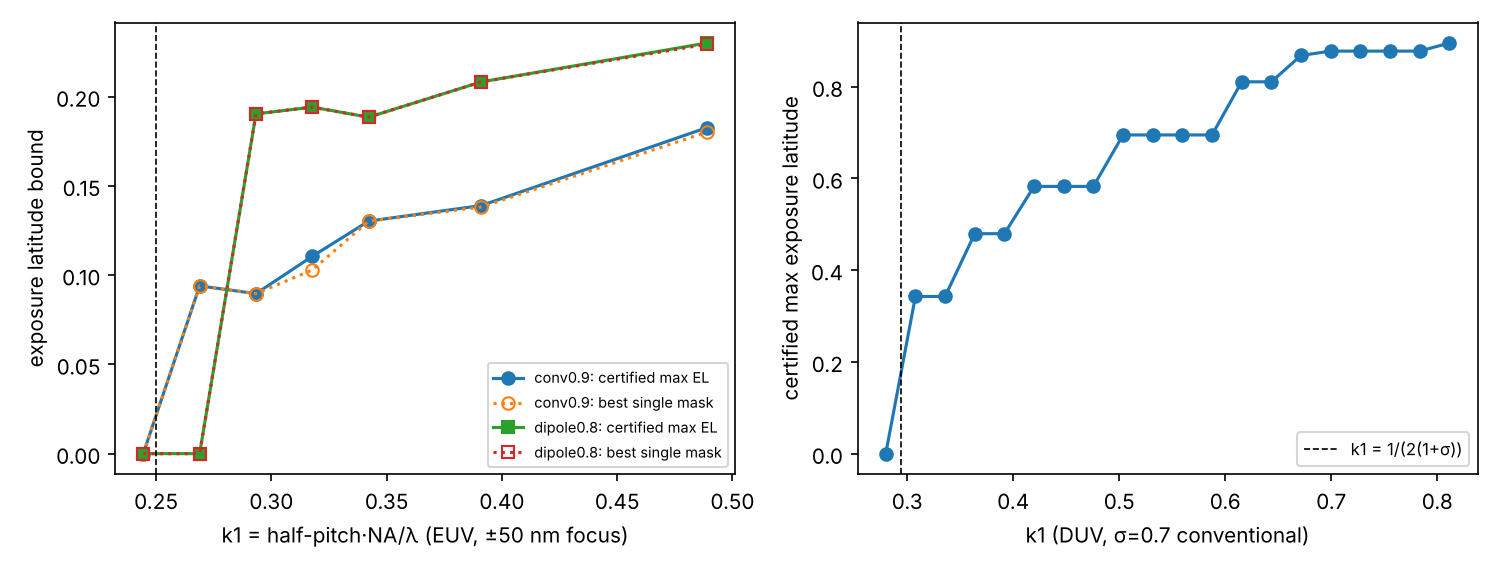
\includegraphics[width=.95\linewidth]{fig2_k1_limits.png}
\caption{Certified maximum exposure latitude versus the normalized half-pitch $k_1=\text{half-pitch}\cdot\NA/\lambda$ for dense lines. Left: EUV ($\lambda=\SI{13.5}{nm}$, $\NA=0.33$) with $\pm\SI{50}{nm}$ focus under conventional $\sigma=0.9$ and dipole $\sigma=0.8$ illumination; the certified bound and the best single mask coincide on every point, and the dashed line marks $k_1=0.25$. Right: DUV ($\lambda=\SI{193}{nm}$, $\NA=1.35$) with conventional $\sigma=0.7$ illumination; the dashed line is the classical cutoff $k_1=1/(2(1+\sigma))$, below which the certified exposure latitude is exactly zero (Proposition~\ref{prop:cutoff}).}\label{fig:k1}\end{figure}

\subsection{One-dimensional feature library}
Dipole and dense-line cases are exactly tight; conventional-illumination gaps are at most 2.5\%; coherent illumination shows large gaps (iso-dense 30.8\%, mixed 13.7\%), and the three-focus cases show gaps of 11--16\% (Table~\ref{tab:1d}). Figure~\ref{fig:cert} shows a certificate for the iso-dense target: the dual weights concentrate on the edge-offset samples, and the interior samples carry zero weight.
\begin{table}[tbp]\centering\small
\caption{One-dimensional feature library (DUV, $\lambda=\SI{193}{nm}$, $\NA=1.35$; edge tolerance $\tau=\SI{8}{nm}$, except \SI{6}{nm} for the dense-90 case). $F$: number of collected orders; foci: $|Z|$, with $\pm\SI{80}{nm}$ denoting the focus set $\{-80,0,+80\}\,\mathrm{nm}$; bound $\rho$: rigorized certificate value (dimensionless dark-to-bright ratio); max EL: $(1-\rho)/(1+\rho)$ at the bound; best single $\rho$: best feasible real mask found; gap $=$ (best single mask $-$ bound)/bound. ``iso-dense'' and ``mixed'' are the isolated-plus-dense and mixed-width line targets; ``dense 90'' is a \SI{90}{nm}-pitch dense-line target, listed for conventional $\sigma=0.7$ / dipole / coherent illumination.}\label{tab:1d}
\resizebox{\linewidth}{!}{\begin{tabular}{lrrrrrr}\toprule
Case & $F$ & Foci & Bound $\rho$ & Max EL & Best single $\rho$ & Gap\\\midrule
iso-dense, coherent & 9 & 1 & 0.3625 & 0.468 & 0.4741 & 30.8\%\\
mixed, coherent & 7 & 1 & 0.4211 & 0.407 & 0.4787 & 13.7\%\\
iso-dense, $\sigma=0.7$ & 15 & 1 & 0.4691 & 0.361 & 0.4808 & 2.5\%\\
mixed, $\sigma=0.7$ & 11 & 1 & 0.4825 & 0.349 & 0.4836 & 0.2\%\\
iso-dense, dipole 0.8 & 15 & 1 & 0.4313 & 0.397 & 0.4313 & 0.0\%\\
mixed, dipole 0.8 & 13 & 1 & 0.4211 & 0.407 & 0.4211 & 0.0\%\\
iso-dense, $\sigma=0.7$, $\pm\SI{80}{nm}$ & 15 & 3 & 0.8131 & 0.103 & 0.9044 & 11.2\%\\
mixed, $\sigma=0.7$, $\pm\SI{80}{nm}$ & 11 & 3 & 0.8691 & 0.070 & 0.9742 & 12.1\%\\
iso-dense, dipole 0.8, $\pm\SI{80}{nm}$ & 15 & 3 & 0.7686 & 0.131 & 0.8921 & 16.1\%\\
dense 90, $\sigma=0.7$ / dipole / coherent & 9/9/5 & 1 & 0.6428/0.4217/0.4217 & 0.217/0.407/0.407 & $=$ bound & 0.0\%\\
\bottomrule\end{tabular}}\end{table}
\begin{figure}[tbp]\centering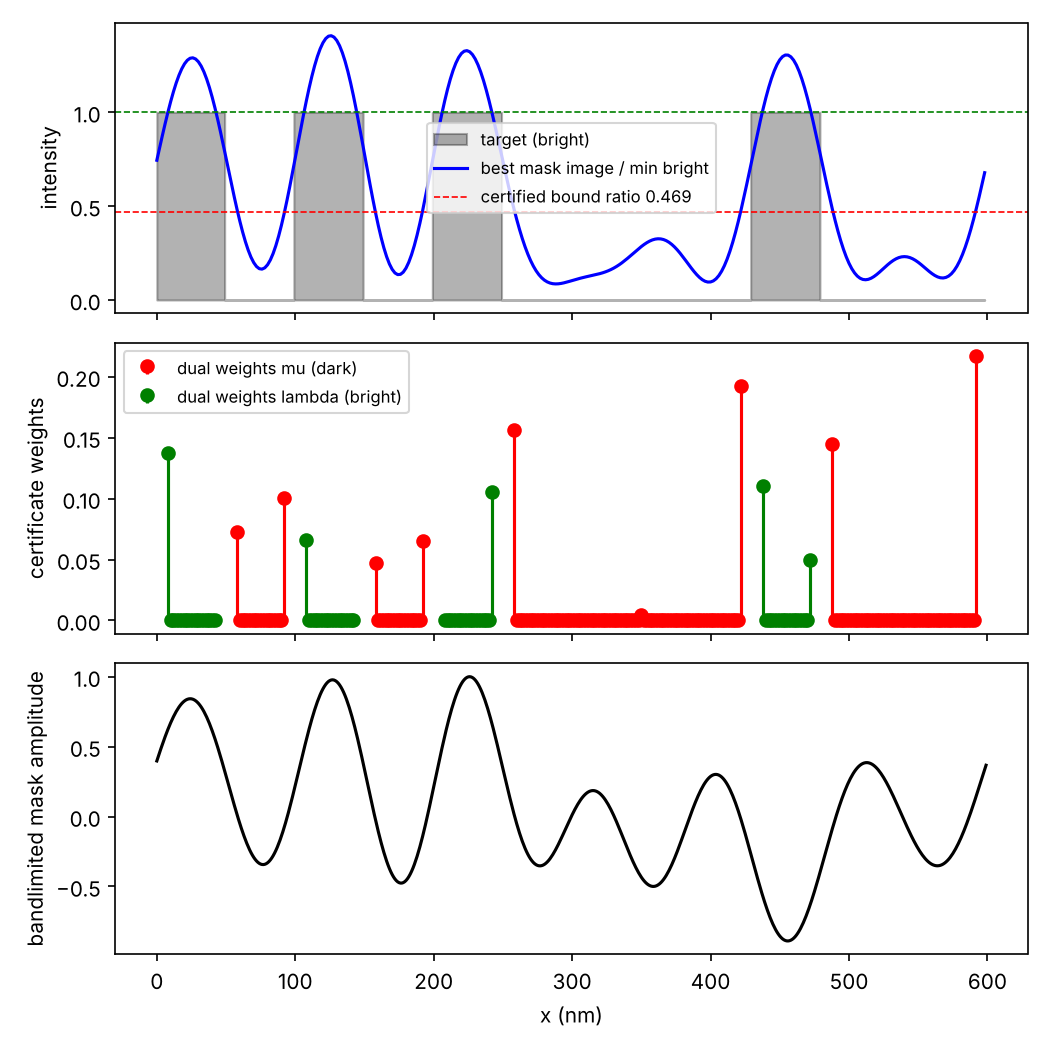
\includegraphics[width=.95\linewidth]{fig1_certificate_isodense.png}
\caption{Certificate for the iso-dense target under conventional $\sigma=0.7$ illumination (DUV, $\NA=1.35$; Table~\ref{tab:1d}). Top: target (gray, bright regions) and the image of the best single mask normalized to its minimum bright intensity; the dashed red line is the certified bound $\rho=0.469$, which no mask can beat. Middle: dual certificate weights $\mu_d$ (dark, red) and $\lambda_b$ (bright, green); the weights concentrate on the edge-offset sample points and vanish on interior samples. Bottom: the band-limited amplitude of the best mask (a phase-shift mask; negative values are $\pi$-phase regions).}\label{fig:cert}\end{figure}

\subsection{Random one-dimensional targets}
On 109 random targets (1--4 segments of width $\ge\SI{40}{nm}$ in 300--\SI{600}{nm} cells; $\tau=\SI{10}{nm}$) the best single mask matches the certified bound to $10^{-4}$ in 69.7\% of instances, to 1\% in 82.6\% and to 5\% in 91.7\% (median gap $1.8\times10^{-6}$, maximum 17.3\%; Table~\ref{tab:random}, Fig.~\ref{fig:gaphist}). Exact tightness is source-dependent (85\% for $\sigma=0.9$, 75\% for the dipole, 57\% for coherent and for $\sigma=0.5$ illumination); every gap above 5\% has minimal optimal-face rank 2 or 3, consistent with Theorem~\ref{thm:me}.
\begin{table}[tbp]\centering\small
\caption{Tightness of the certified bound on 109 random one-dimensional targets (DUV, $\NA=1.35$; 1--4 segments of width $\ge\SI{40}{nm}$ in 300--\SI{600}{nm} cells; $\tau=\SI{10}{nm}$). Gap $=$ (best single mask $-$ bound)/bound. ``Exactly tight'' means gap $\le10^{-4}$. The per-source rows give the fraction of exactly tight instances for each illumination.}\label{tab:random}
\begin{tabular}{@{}lr@{}}\toprule
Criterion & Fraction of instances\\\midrule
gap $\le10^{-4}$ (exactly tight) & 69.7\%\\
gap $\le1\%$ & 82.6\%\\
gap $\le5\%$ & 91.7\%\\
median gap / maximum gap & $1.8\times10^{-6}$ / 17.3\%\\
\midrule
exactly tight, conventional $\sigma=0.9$ & 85\%\\
exactly tight, dipole & 75\%\\
exactly tight, coherent & 57\%\\
exactly tight, conventional $\sigma=0.5$ & 57\%\\
\bottomrule\end{tabular}\end{table}
\begin{figure}[tbp]\centering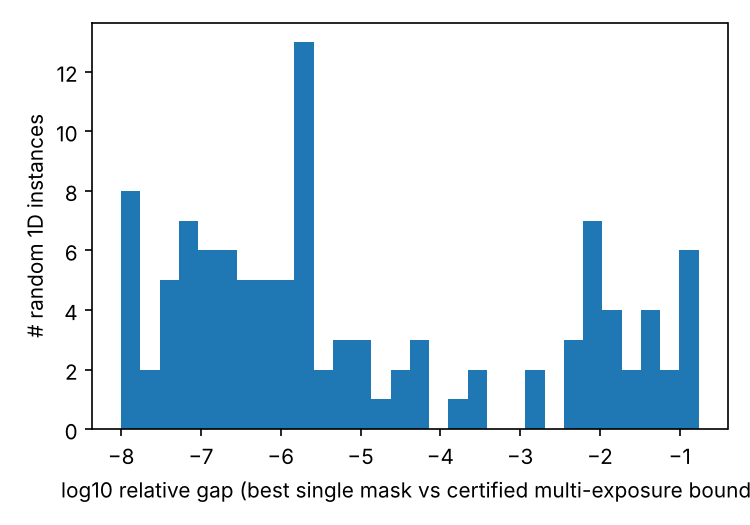
\includegraphics[width=.6\linewidth]{fig3_gap_hist.png}
\caption{Histogram of $\log_{10}$ of the relative gap between the best single mask and the certified multi-exposure bound over the 109 random one-dimensional targets of Table~\ref{tab:random}. The population is bimodal: most instances are tight to solver precision (gap $\lesssim10^{-5}$), while the instances with gaps of $10^{-2}$--$10^{-1}$ have optimal-face rank 2 or 3 (Theorem~\ref{thm:me}).}\label{fig:gaphist}\end{figure}

\subsection{Certified multi-exposure gains}
Theorem~\ref{thm:bnb} converges in \SIrange{0.3}{1.6}{s} for $F=5$ and proves the gains of Table~\ref{tab:bnb} (Fig.~\ref{fig:bnb}, left); each optimal face has rank 2, so two exposures suffice. The Lasserre-2 single-mask bounds coincide with $U$ to $10^{-6}$ on these instances (cross-checked between CLARABEL, 0.4787045, and SCS, 0.4787037, on the mixed target). For $F=9$ (iso-dense, coherent) and $F=11$ (three-focus mixed target) the interval branch-and-bound does not converge within $6\times10^6$ nodes; only Lasserre-2 values (0.4608 and 0.9552, solver status \emph{optimal\_inaccurate}) corroborate gains of 27\% and 9.9\%, which we therefore do not count as certified.
\begin{table}[tbp]\centering\small
\caption{Rigorous separation of single- and multi-exposure optima by the interval branch-and-bound of Theorem~\ref{thm:bnb} (DUV, coherent illumination). $F$: collected orders; SDP bound: rigorized certificate value $t_R$ (optimum over any number of exposures); B\&B $L$: certified lower bound on the single-mask optimum $\rhostar(\mathcal M_\R)$; best single $U$: incumbent, so that $L\le\rhostar(\mathcal M_\R)\le U$; nodes: branch-and-bound nodes explored; converged: whether $L\ge(1-\mathrm{tol})U$ was reached; certified gain $=(L-\text{SDP bound})/\text{SDP bound}$, a rigorous lower bound on the multi-exposure improvement in $\rho$. ``random $n$'' are instances of the random one-dimensional set.}\label{tab:bnb}
\resizebox{\linewidth}{!}{\begin{tabular}{lrrrrrrr}\toprule
Case & $F$ & SDP bound & B\&B $L$ & Best single $U$ & Nodes & Converged & Certified gain\\\midrule
random 82 (coherent) & 5 & 0.3597 & 0.4061 & 0.4066 & 40,383 & yes & 12.9\%\\
random 91 (coherent) & 5 & 0.6049 & 0.6775 & 0.6782 & 76,027 & yes & 12.0\%\\
random 110 (coherent) & 5 & 0.3464 & 0.4033 & 0.4037 & 17,413 & yes & 16.4\%\\
random 50 (coherent) & 5 & 0.3141 & 0.3343 & 0.3347 & 28,517 & yes & 6.4\%\\
mixed (coherent) & 7 & 0.4211 & 0.4776 & 0.4787 & $3.0\times10^7$ & no (0.23\% gap) & 13.4\%\\
\bottomrule\end{tabular}}\end{table}
\begin{figure}[tbp]\centering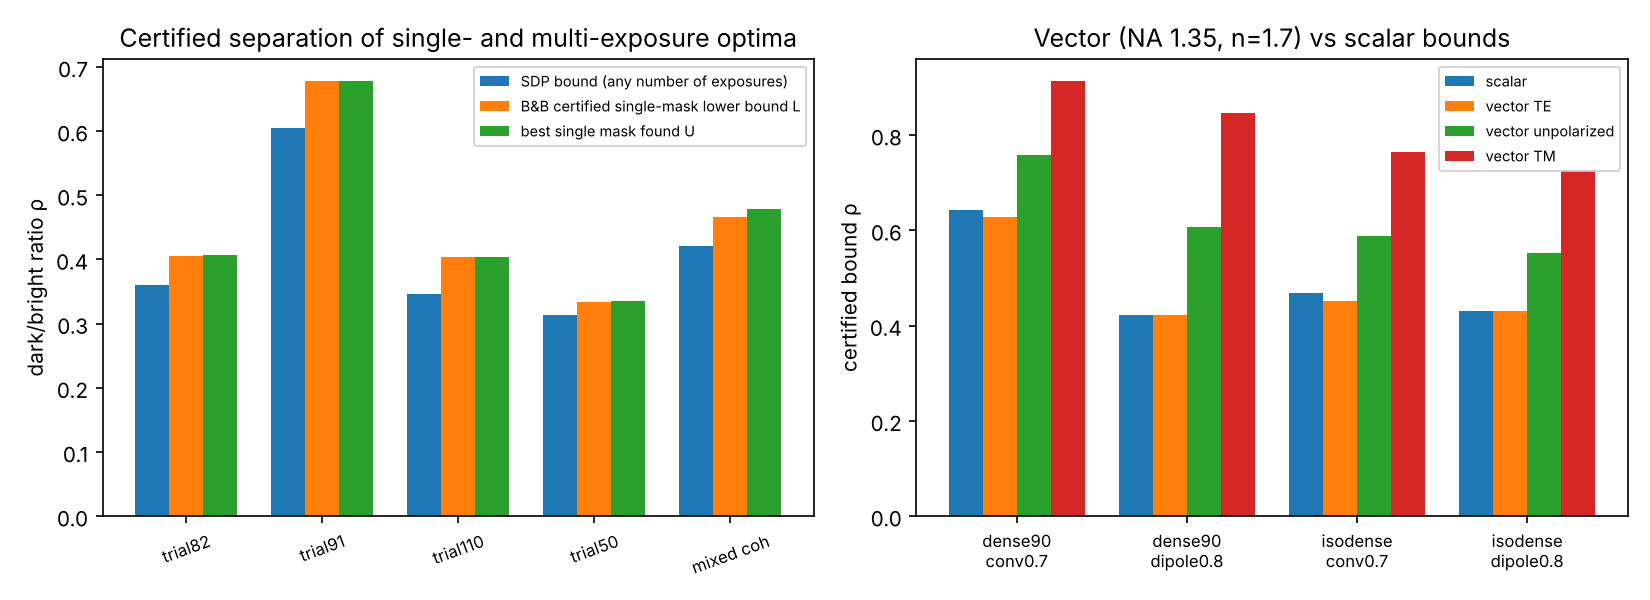
\includegraphics[width=\linewidth]{fig5_bnb_vector.png}
\caption{Left: certified separation of single- and multi-exposure optima (Table~\ref{tab:bnb}). For each case the bars show the SDP bound $t_R$ (valid for any number of exposures), the branch-and-bound certified single-mask lower bound $L$, and the best single mask found $U$; a visible gap between the first bar and the second proves that multiple exposure strictly improves the ratio. For the two large-$F$ cases (iso-dense coherent; mixed, $\sigma=0.7$, $\pm\SI{80}{nm}$) the branch-and-bound did not converge and $L$ is not informative. Right: certified bounds $\rho$ under the scalar model and under the vector model ($\NA=1.35$, resist index $n=1.7$) for TE, unpolarized and TM illumination on four one-dimensional targets (\S\ref{sec:robust}).}\label{fig:bnb}\end{figure}

\subsection{Phase-shift versus binary masks and pattern-error ILT}
Table~\ref{tab:psm} compares the certified optima of phase-shift (PSM) and binary masks with the results of a standard pattern-error ILT on the iso-dense, mixed and dense-120 targets ($\sigma=0.7$, $\tau=\SI{10}{nm}$). The DNN relaxation for nonnegative masks gives 0.4266/0.4599/0.3777 against PSM bounds of 0.3879/0.4031/0.3671: binary masks forfeit a certified 10\%/14\%/3\%. Pixel- and Fourier-domain PSM relaxations agree to $10^{-5}$. A standard pattern-error ILT (sigmoid resist, open-frame-normalized intensity, threshold 0.3, best of six settings, 1,500 Adam steps, gradient verified by finite differences) reaches 0.553/0.672/0.477 (PSM) and 0.579/0.722/0.517 (binary), i.e.\ 30--67\% (PSM) and up to 79\% (binary) above the certified PSM optimum. Refining the ILT mask on the ratio objective closes the gap on dense-120 (0.3671) and partially elsewhere (0.426 and 0.530).
\begin{table}[tbp]\centering\small
\caption{Certified phase-shift (PSM) and binary-mask optima versus a standard pattern-error ILT (DUV, $\NA=1.35$, conventional $\sigma=0.7$, $\tau=\SI{10}{nm}$). All entries are dark-to-bright ratios $\rho$ (lower is better). PSM bound: rigorized SDP certificate over real masks; binary bound: doubly-nonnegative (DNN) relaxation over nonnegative masks; binary penalty: certified relative increase of the binary bound over the PSM bound; ILT (PSM/binary): ratio reached by the pattern-error ILT mask; ILT refined: the ILT mask after local refinement on the ratio objective. ``dense 120'' is a \SI{120}{nm}-pitch dense-line target.}\label{tab:psm}
\begin{tabular}{@{}lrrrrrr@{}}\toprule
Target & PSM bound & Binary bound & Binary penalty & ILT (PSM) & ILT (binary) & ILT refined\\\midrule
iso-dense & 0.3879 & 0.4266 & 10\% & 0.553 & 0.579 & 0.426\\
mixed & 0.4031 & 0.4599 & 14\% & 0.672 & 0.722 & 0.530\\
dense 120 & 0.3671 & 0.3777 & 3\% & 0.477 & 0.517 & 0.3671\\
\bottomrule\end{tabular}\end{table}

\subsection{Source--mask entitlement}
For the iso-dense target the per-source-point relaxation equals the coherent bound (0.3625) both for $\sigma=0.7$ and for a 13-point $\sigma=0.9$ grid, whereas the fixed-source bounds are 0.43--0.51: no illumination supported on these points beats on-axis coherent light for this metric.

\subsection{Two-dimensional layouts}
Contact arrays are certified essentially tight with rank-one optima (Table~\ref{tab:2d}). For the \SI{320}{nm} cells ($F=61$, approximately 1,200 constraints) the strong search closes the annular T-junction and the line-end gaps to $0.61\%$ and $0.03\%$ (Fig.~\ref{fig:2d}); the quasar T-junction retains a 6.2\% gap that we could neither close nor certify as a multi-exposure gain (the interval branch-and-bound is out of reach at $F=61$, and a two-exposure local refinement did not beat the single mask). The weighted dark matrix has a four-dimensional common null space (orders invisible to every constraint); the certificate is verified on its complement. On 40 random two-rectangle layouts in 200--\SI{240}{nm} cells (annular, quasar and $\sigma=0.5$ illumination; $F=13$--37) the single-mask search matches the bound to $10^{-3}$ in 45\% and to 5\% in 62.5\% of cases; the remaining gaps (up to 26\%, mostly for $\sigma=0.5$ and $F=37$) are unresolved upper bounds on the multi-exposure benefit (Fig.~\ref{fig:dataset}, left). EUV contact arrays (32--\SI{44}{nm} pitch, $\pm\SI{40}{nm}$ focus) are tight, with certified EL from 0.13 to 0.41 (Fig.~\ref{fig:dataset}, right).
\begin{table}[tbp]\centering\small
\caption{Two-dimensional layouts (DUV, $\lambda=\SI{193}{nm}$, $\NA=1.35$). Contact arrays: pitch in nm as given in the case name, with edge tolerance $\tau=12$, 10 and \SI{8}{nm} for 160, 120 and \SI{100}{nm} pitch respectively; T-junction and line-end cells: \SI{320}{nm} cell, $\tau=\SI{14}{nm}$. $F$: collected orders; bound $\rho$: rigorized certificate value; max EL: $(1-\rho)/(1+\rho)$ at the bound; best single $\rho$: best feasible real mask found; gap $=$ (best single mask $-$ bound)/bound; SDP time: wall-clock time of the relaxation solve in seconds. ``strong'': 12-start search with vectorized SLSQP polish.}\label{tab:2d}
\resizebox{\linewidth}{!}{\begin{tabular}{lrrrrrr}\toprule
Layout & $F$ & Bound $\rho$ & Max EL & Best single $\rho$ & Gap & SDP time\\\midrule
contacts 160, annular & 13 & 0.5843 & 0.262 & 0.5861 & 0.30\% & \SI{1.4}{s}\\
contacts 160, $\sigma=0.5$ & 9 & 0.6174 & 0.237 & 0.6177 & 0.04\% & \SI{1.5}{s}\\
contacts 120, annular & 9 & 0.6957 & 0.179 & 0.6962 & 0.07\% & \SI{0.7}{s}\\
contacts 120, quasar & 9 & 0.5740 & 0.271 & 0.5747 & 0.13\% & \SI{0.7}{s}\\
contacts 100, quasar & 5 & 0.8751 & 0.067 & 0.8754 & 0.03\% & \SI{0.5}{s}\\
T-junction 320, annular (strong) & 61 & 0.4387 & 0.390 & 0.4413 & 0.61\% & \SI{410}{s}\\
T-junction 320, quasar (strong) & 61 & 0.3893 & 0.440 & 0.4135 & 6.2\% & \SI{269}{s}\\
line-ends 320, annular (strong) & 61 & 0.5194 & 0.316 & 0.5195 & 0.03\% & \SI{649}{s}\\
\bottomrule\end{tabular}}\end{table}
\begin{figure}[tbp]\centering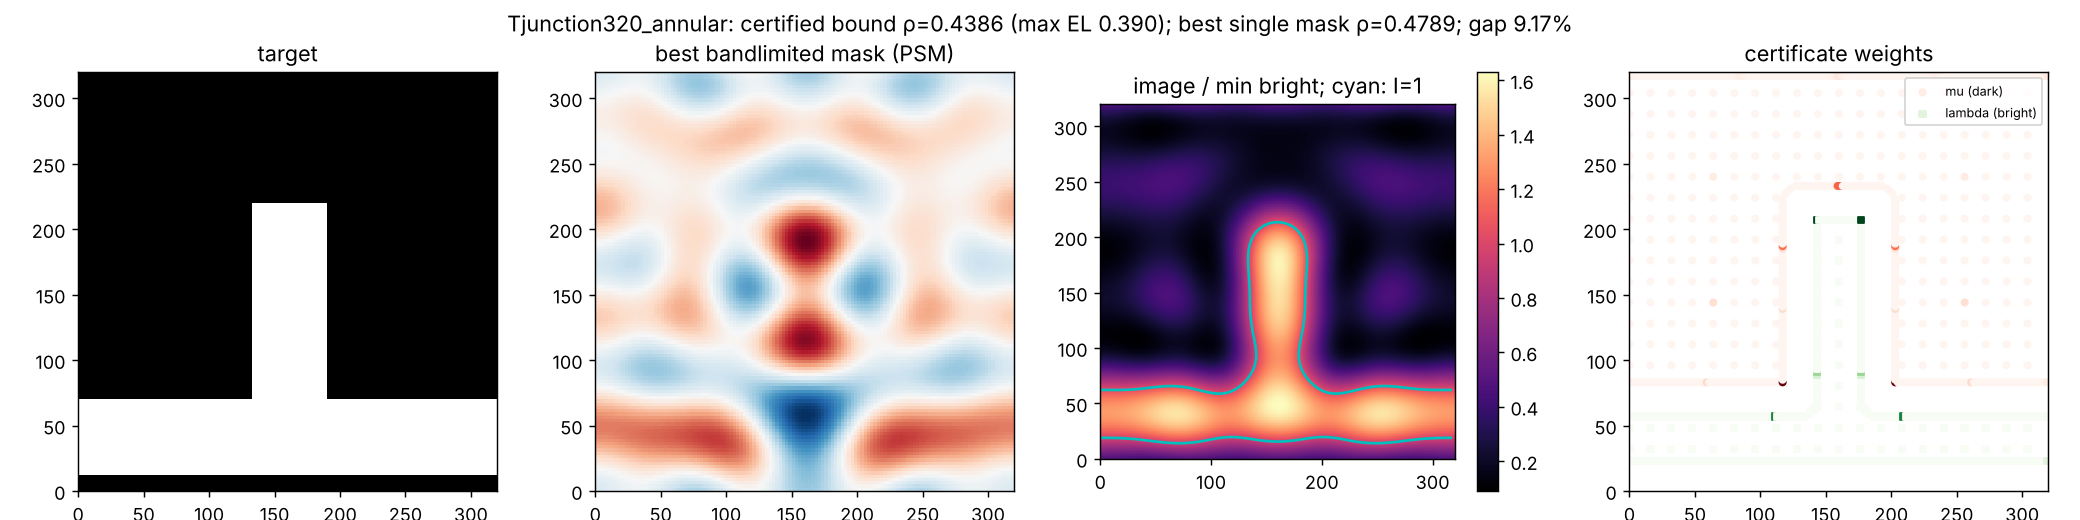
\includegraphics[width=\linewidth]{fig4_2d_Tjunction.png}
\caption{T-junction in a \SI{320}{nm} cell under annular illumination (DUV, $\NA=1.35$, $\tau=\SI{14}{nm}$; axes in nm). From left to right: the target (white = bright); the best band-limited phase-shift mask (signed amplitude); the normalized image with the $\I=1$ contour (cyan), which traces the printed feature; and the certificate weights $\mu_d$ (dark) and $\lambda_b$ (bright), which localize the limiting corners and the line-end. The certified bound is $\rho=0.4387$ (maximum EL 0.390). The mask shown is from the baseline search ($\rho=0.4789$, as in the panel title); the strong search of Table~\ref{tab:2d} reaches $\rho=0.4413$ (gap 0.61\%) against the same certificate.}\label{fig:2d}\end{figure}
\begin{figure}[tbp]\centering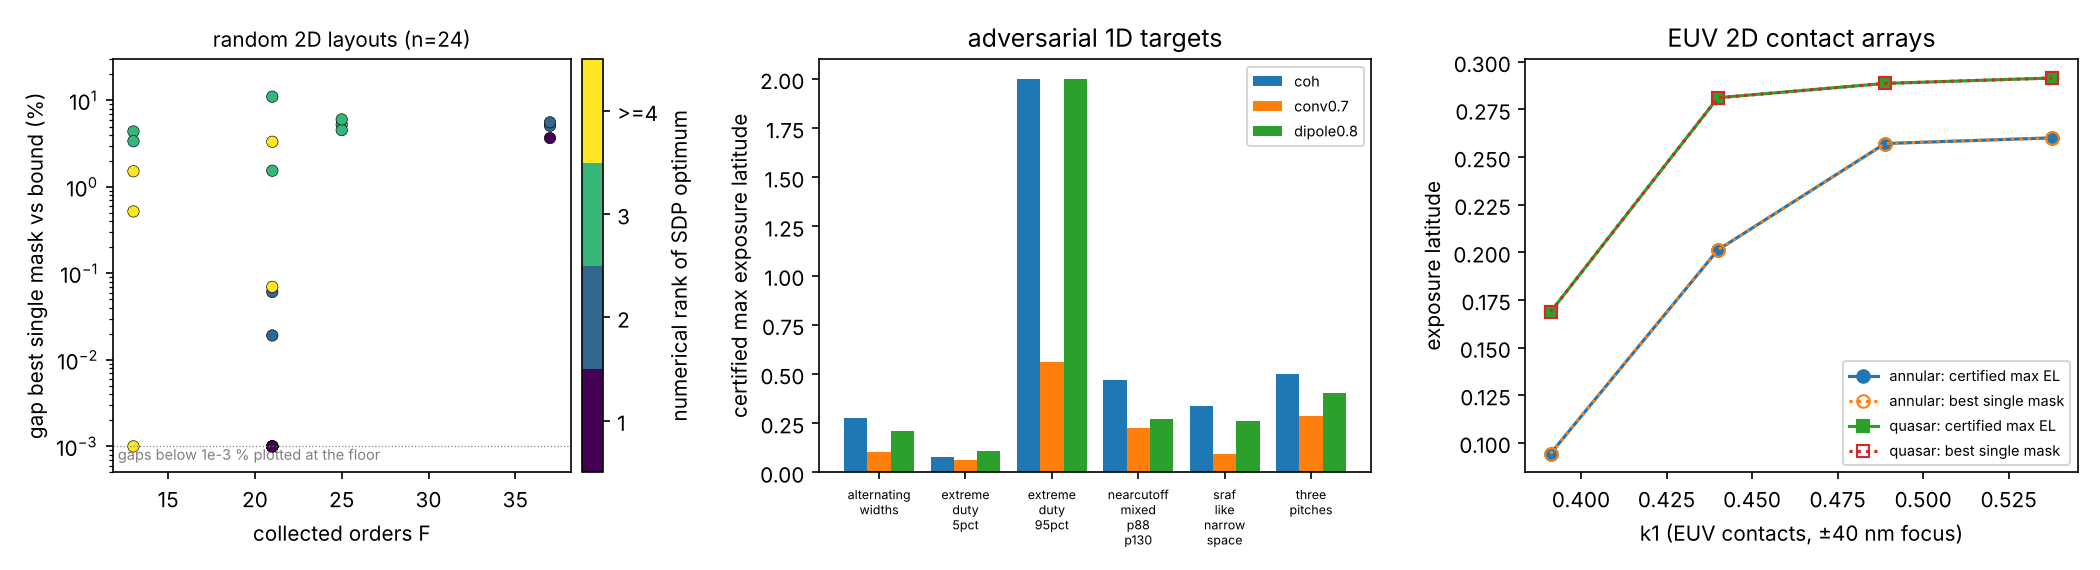
\includegraphics[width=\linewidth]{fig6_dataset.png}
\caption{Expanded dataset. Left: gap between the best single mask and the certified bound (percent, logarithmic scale) versus the number of collected orders $F$ for 40 random two-rectangle two-dimensional layouts; the marker color encodes the rank of the SDP optimum (dark = rank one). Middle: certified maximum exposure latitude of the adversarial one-dimensional targets of \S\ref{sec:adv} under coherent (``coh''), conventional $\sigma=0.7$ (``conv0.7'') and dipole $\sigma=0.8$ (``dipole0.8'') illumination. Right: EUV two-dimensional contact arrays (32--\SI{44}{nm} pitch, $\pm\SI{40}{nm}$ focus) under annular and quasar illumination; the certified maximum EL and the best single mask coincide at every $k_1$.}\label{fig:dataset}\end{figure}

\subsection{Adversarial one-dimensional targets}\label{sec:adv}
Near-cutoff mixed pitches, SRAF-like \SI{20}{nm} spaces, 5\%/95\% duty cycles, alternating widths and three-pitch mixtures (Fig.~\ref{fig:dataset}, middle) are tight under dipole illumination, mostly tight under $\sigma=0.7$, and show 12--37\% gaps under coherent illumination (rank 3--5), the regime in which multiple exposure helps most. The isolated \SI{20}{nm} space under coherent or dipole light has a certified bound of $\approx0$: a phase-edge mask prints an arbitrarily dark narrow line, which the relaxation recognizes.

\subsection{Robustness, solver validation and physical sensitivity}\label{sec:robust}
Table~\ref{tab:sens} summarizes the sensitivity studies. The bound is invariant to the interior sample spacing and monotone in the edge tolerance $\tau$; the source quadrature converges; the Rayleigh-quotient bound is 1--148$\times$ weaker (Table~\ref{tab:rayleigh}); and the complex- and real-mask relaxations coincide on all nine cases (Lemma~\ref{lem:complex}). All 136 reported bounds were recomputed and their projected certificate matrices factorized exactly by a 50-digit Cholesky (135 succeed; the remaining EUV case, with bound exactly 1, has $S=0$, Proposition~\ref{prop:cutoff}); the rigorization scale $\kappa$ exceeds 0.99999 except on one near-degenerate random instance (bound $10^{-3}$, $\kappa=0.835$). CLARABEL and SCS agree to a median of $7\times10^{-9}$; on five near-degenerate random instances (bounds $\le10^{-2}$) SCS is off by up to 0.14 and once negative, which the certificate check exposes. Under the vector model ($n_{\mathrm{resist}}=1.7$) the TE bounds are 0--4\% below the scalar ones, the unpolarized bounds 10--40\% above and the TM bounds 70--120\% above (the classical TM contrast loss at $\NA=1.35$), with tightness unchanged (Fig.~\ref{fig:bnb}, right); aberrations of 0.02--0.1$\lambda$ move the iso-dense bound by 0--7\%; pixelation at $N\ge F$ leaves it unchanged and coarser pixels raise it (+15\% at \SI{50}{nm}, +46\% at \SI{67}{nm}), as Lemma~\ref{lem:pixel} predicts.
\begin{table}[tbp]\centering\small
\caption{Sensitivity of the certified bound and solver validation (DUV, $\NA=1.35$; one-dimensional targets of Table~\ref{tab:1d} unless stated). Percentages are relative changes of the bound $\rho$ with respect to the reference setting in the second column; EL is the exposure latitude $(1-\rho)/(1+\rho)$; $\kappa$ is the rigorization scale of \S\ref{sec:alg}.}\label{tab:sens}
\begin{tabular}{@{}>{\raggedright\arraybackslash}p{0.31\linewidth}>{\raggedright\arraybackslash}p{0.19\linewidth}>{\raggedright\arraybackslash}p{0.43\linewidth}@{}}\toprule
Study & Setting varied & Effect on the bound\\\midrule
interior sample spacing & 16 to \SI{1}{nm} & invariant (0.46907 throughout)\\
edge tolerance $\tau$ & 2 to \SI{20}{nm} & monotone: max EL 0.09 to 0.74\\
source quadrature & 11 to 21 source points & converges: 0.513 to 0.526\\
complex- versus real-mask relaxation & nine cases & coincide (Lemma~\ref{lem:complex}; Table~\ref{tab:rayleigh})\\
Rayleigh-quotient bound & six cases & 1--148$\times$ weaker (Table~\ref{tab:rayleigh})\\
vector model, TE ($n_{\mathrm{resist}}=1.7$) & versus scalar & 0--4\% lower; tightness unchanged\\
vector model, unpolarized & versus scalar & 10--40\% higher\\
vector model, TM & versus scalar & 70--120\% higher (TM contrast loss)\\
pupil aberrations & 0.02--0.1$\lambda$ & iso-dense bound moves by 0--7\%\\
pixelation & $N\ge F$ pixels per period & unchanged (Lemma~\ref{lem:pixel})\\
pixelation & 50 / \SI{67}{nm} pixels & +15\% / +46\%\\
\midrule
50-digit Cholesky of certificate & 136 bounds & 135 factorize; one has $S=0$ (bound 1)\\
rigorization scale $\kappa$ & 136 bounds & $>0.99999$, except one instance with $\kappa=0.835$ (bound $10^{-3}$)\\
CLARABEL versus SCS & all instances & median difference $7\times10^{-9}$; five near-degenerate instances (bounds $\le10^{-2}$) off by up to 0.14, once negative\\
\bottomrule\end{tabular}\end{table}
\begin{table}[tbp]\centering\small
\caption{Certified SDP bound (real masks) versus the generalized-eigenvalue (Rayleigh-quotient) bound and the complex-mask relaxation on one-dimensional targets (DUV, $\NA=1.35$, $\tau=\SI{8}{nm}$; dense 90: \SI{6}{nm}). All entries are lower bounds on the dark-to-bright ratio $\rho$ (higher is tighter); $F$: collected orders. The complex-mask relaxation coincides with the real-mask one in every case (Lemma~\ref{lem:complex}).}\label{tab:rayleigh}
\begin{tabular}{@{}llrrrr@{}}\toprule
Case & Source & $F$ & SDP (real) & Rayleigh & SDP (complex)\\\midrule
iso-dense & coherent & 9 & 0.3625 & 0.0668 & 0.3625\\
iso-dense & $\sigma=0.7$ & 15 & 0.4691 & 0.1387 & 0.4691\\
iso-dense & dipole & 15 & 0.4313 & 0.0823 & 0.4313\\
mixed & coherent & 7 & 0.4211 & 0.0028 & 0.4211\\
mixed & $\sigma=0.7$ & 11 & 0.4825 & 0.0343 & 0.4825\\
dense 90 & $\sigma=0.7$ & 9 & 0.6428 & 0.4392 & 0.6428\\
\bottomrule\end{tabular}\end{table}

\FloatBarrier
\section{Discussion}
The certificates turn folklore into checkable statements. Local optimization of the exposure-latitude objective is globally optimal for most one-dimensional targets and for the two-dimensional contact arrays; when it is not, the shortfall is---by Theorem~\ref{thm:me}---the benefit of incoherent multiple exposure, which Theorem~\ref{thm:bnb} proves to be strictly positive on concrete coherent-illumination targets. Coherent illumination with phase-shift masks is the certified entitlement for the iso-dense target, and binary masks forfeit a certified 3--14\%. Pattern-error ILT is far from EL-optimal, which argues for EL or contrast objectives, or for the certificate as a stopping criterion. The dual weights localize the limiting geometry. These conclusions survive the vector model and moderate aberrations. Finally, the relaxation gap has a physical meaning and is therefore informative rather than merely a weakness.

\section{Limitations}
The model is a thin-mask periodic model (no three-dimensional mask electromagnetics, resist chemistry, flare or mask error) with sampled constraints and an explicit edge tolerance. The objective is the ratio/EL objective (any constraint linear in intensity lifts identically; edge-placement error enters only through $\tau$). The DNN relaxation is only an outer approximation in two dimensions; Lasserre-2 values carry a solver status and are not counted as certificates; the branch-and-bound converges only for $F\le7$; one \SI{320}{nm} two-dimensional gap (6.2\%) and the large-$F$ random two-dimensional gaps remain unresolved; and near-degenerate instances (bound $\lesssim10^{-2}$) stress first-order solvers. Literature verification relied on abstracts and search snippets (the full texts of \cite{rosenbluth2002,rosenbluth2007,liu1992} were not accessible).

\section*{Data and Code Availability}
All code, data and the complete verification record accompany this manuscript in the repository directories \texttt{code/}, \texttt{results/} and \texttt{notes/}. The pipeline depends only on open-source Python packages (\texttt{pip install numpy scipy cvxpy matplotlib mpmath}). Running \texttt{cd code \&\& python3 -W ignore test\_certlitho.py} executes the nine unit tests, and \texttt{./run\_all\_par.sh} regenerates every table and figure of this manuscript from scratch (about 3.5 hours on four cores). The JSON outputs, solver logs and the table source \texttt{results/RESULTS\_TABLES.md} are stored in \texttt{results/}.

\section*{Acknowledgements and Competing Interests}
This manuscript was prepared by an autonomous research system under human oversight; the human overseers reviewed the claims, the verification record and the final text. No external funding was received for this work. The authors declare no competing interests.

\bibliographystyle{unsrtnat}
\bibliography{refs}
\end{document}
